\section{Afstandssensor}

Udgangspunktet for denne undersøgelse er så vidt som muligt at bruge de komponenter vi har til rådighed i Embedded Stock. Hvilket umiddelbart betyder en Ultra Sonisk sensor af typen:

\begin{table}[H] \centering
\begin{tabular}{|p{3cm}|p{11cm}|}
	\hline
	\textbf{Løsning}		
	    & HC-SR04 Ultra Sonic Sensor
	\\ \hline
	\textbf{Producent} 		
	    & Elec Freaks
	\\ \hline
	\textbf{Interface} 		
	    & TTL\footcite{ttl}
	\\ \hline
	\textbf{Beskrivelse} 	
	    & Sensoren trigges med en 10uS TTL puls, hvorefter sensoren udsender et sonar signal på 40kHz. Output fra sensoren er en TTL puls af samme varighed som det tager Sensoren at modtage et ekko
	\\ \hline
	\textbf{Krav} 			
	    & Godt kendskab til PSoC creator
	\\ \hline
	\textbf{Fordele}		
	    & Denne sensor kræver ingen ekstra HW. Den er simpel i brug, stabil og præcis
	\\ \hline
	\textbf{Ulemper} 		
	    & Begrænset målevinkel
	\\ \hline
	\textbf{Pris} 			
	    & Ved lavpris elektronik: 59,- (Hentet gratis på EL-lab)
	\\ \hline
	\textbf{Link} 			
	    & \url{http://www.micropik.com/PDF/HCSR04.pdf}
	\\ \hline
	\multicolumn{2}{|c|}{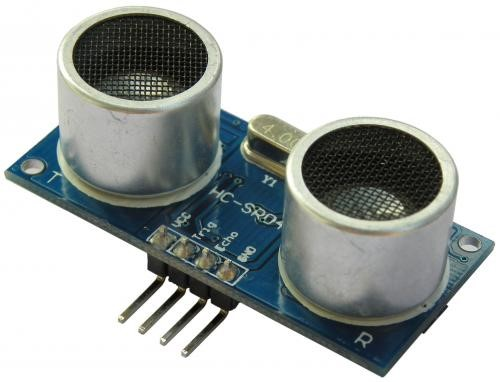
\includegraphics[width=0.3\linewidth]{0_Filer/Figuer/Forudundersoegelse/Afstandssensor_billede.jpg}}
    \\ \hline
\end{tabular}
\end{table}

\subsection{Konklusion}

HC-SR04 Ultra Sonic sensor opfylder alle de behov der er brug for til projektet. Den er stabil og præcis og kræver ikke ekstra hardware. Da sensoren er tilgængelig på Embedded stock, er denne blevet valgt.
